\documentclass[11pt,a4paper]{article}

\usepackage[T1]{fontenc}
\usepackage[utf8]{inputenc}
\usepackage[english]{babel}
\usepackage{amsmath,amssymb,mathtools}
\usepackage{geometry}
\usepackage{graphicx}
\usepackage{booktabs}
\usepackage{hyperref}
\usepackage{enumitem}
\usepackage{float}

\geometry{margin=2.5cm}
\emergencystretch=2em

\hypersetup{
    colorlinks=true,
    hypertexnames=false,
    linkcolor=blue,
    citecolor=blue,
    urlcolor=blue
}

\graphicspath{{../experiments/active_respect_significance/outputs/}{outputs/}}

\newcommand{\dd}{\mathrm{d}}
\newcommand{\Rresp}{R_{\mathrm{resp}}}
\newcommand{\Rrob}{R_{\mathrm{rob}}}
\newcommand{\Rsig}{R_{\mathrm{sig}}}
\newcommand{\Seff}{S_{\mathrm{eff}}}

\title{
\textbf{Active Structural Significance}\\[0.4em]
\large A Toy Extension of the MAAT v1.2.1 Robustness Closure\\[0.3em]
\small MAAT Structural Selection Series --- Paper 44 / Diagnostic Note
}

\author{
Christof Krieg\\
\small MAAT Project -- Independent Research\\
\small \url{https://maat-research.com}
}

\date{2026}

\begin{document}

\maketitle

\begin{abstract}
MAAT v1.2.1 removed robustness/respect as an independent primitive sector and
reformulated it as an emergent closure over the four primary support sectors
$(H,B,S,V)$.
This move avoided double counting and clarified the role of robustness in
the structural-selection functional.
However, the resulting closure primarily describes passive adherence and
activity-sensitive robustness, not the broader notion of active structural
significance.

This paper introduces a toy extension that preserves the v1.2.1 architecture
while distinguishing three emergent levels:
\[
\Rresp=(HBV)^{1/3},
\qquad
\Rrob=\min\!\left(\Rresp,(HB\Seff V)^{1/4}\right),
\qquad
\Rsig=\Rresp^{1-\alpha}\Seff^\alpha .
\]
Here $\Seff$ is not raw activity but controlled activity in an optimal
window,
\[
\Seff(A)=
\exp\!\left[
-\frac12
\left(\frac{A-A_\star}{\sigma_A}\right)^2
\right].
\]

A reproducible toy simulation with a fixed random seed generates a noisy
$6000$-sample ensemble and shows that passive structural adherence and active
structural significance separate cleanly.
Dormant coherent systems retain moderate passive adherence
($\Rresp\simeq0.636$) but low active significance
($\Rsig\simeq0.098$), while the stable-star archetype reaches
$\Rsig\simeq0.992$.
Across the ensemble, $13.07\%$ of configurations have high $\Rresp$ but low
$\Rsig$.
This supports the distinction between passive respect and active
significance.

The result is not a physical stellar model and not a new primitive-field
proposal.
It supports a cautious interpretation: MAAT v1.2.1 is a robustness closure,
whereas $\Rsig$ is a candidate diagnostic extension for active structural
significance.
\end{abstract}

\tableofcontents

% ------------------------------------------------------------
\section{Purpose and Status}

The v1.2.1 closure clarified an important point:
\[
H,\;B,\;S,\;V
\quad\text{are primary support sectors,}
\]
while robustness is reconstructed as an emergent quantity.
This avoids returning to a five-sector primitive functional of the form
\[
F_{\mathrm{MAAT}}
=
-\sum_{a\in\{H,B,S,V,R\}}
\lambda_a\log(\epsilon+\Gamma_a),
\]
which risks double counting because $R$ is strongly dependent on the other
sectors.

The present paper does not undo that closure.
Instead, it asks a narrower question:
\begin{quote}
\emph{Can the emergent $R$ hierarchy be extended to distinguish passive
robustness from active structural significance?}
\end{quote}

The motivation is simple.
A system may be coherent and constraint-compatible without being dynamically
significant.
Conversely, raw activity alone does not imply significance; excessive activity
can be chaotic.
The missing object is therefore not raw activity, but controlled activity that
remains coherent, balanced, and connected.

This paper is a toy conceptual benchmark.
It should be read as a candidate extension, not as a modification of Papers
36--43.

% ------------------------------------------------------------
\section{Emergent Respect Hierarchy}

The v1.2.1 passive adherence closure is
\begin{equation}
\boxed{
\Rresp=(HBV)^{1/3}.
}
\label{eq:rresp}
\end{equation}
It measures structural compatibility among coherence, balance, and
connectedness.

The activity-sensitive robustness closure is
\begin{equation}
\boxed{
\Rrob=
\min\!\left(
\Rresp,\,
(HB\Seff V)^{1/4}
\right).
}
\label{eq:rrob}
\end{equation}
In earlier v1.2.1 papers the role of $S$ in this boundary was to ensure that
robustness cannot ignore activity.
For the present toy extension, the activity support entering the robustness
boundary is represented by $\Seff$ rather than by a raw activity variable.
This is a toy-level diagnostic convention, not a retroactive change of the
v1.2.1 papers.

The new candidate diagnostic is active structural significance:
\begin{equation}
\boxed{
\Rsig
=
\Rresp^{1-\alpha}\Seff^\alpha,
\qquad
0<\alpha<1.
}
\label{eq:rsig}
\end{equation}
This is not a fifth primitive sector.
It is an observable constructed from the passive adherence closure and the
controlled-activity support.
Thus $\Rsig$ measures not whether a system merely satisfies its constraints,
but whether its constraint-compatible structure becomes dynamically
effective.

% ------------------------------------------------------------
\section{Controlled Activity}

Raw activity $A$ is not automatically beneficial.
Too little activity produces dormant coherence; too much activity produces
chaotic overdrive.
The toy model therefore defines an effective controlled-activity support:
\begin{equation}
\boxed{
\Seff(A)
=
\exp\!\left[
-\frac12
\left(\frac{A-A_\star}{\sigma_A}\right)^2
\right].
}
\label{eq:seff}
\end{equation}
The benchmark parameters are
\begin{equation}
A_\star=1.0,
\qquad
\sigma_A=0.28,
\qquad
\alpha=0.45.
\end{equation}

This implements the intended interpretation:
\begin{quote}
\emph{Significance is generated by activity inside a coherent control window,
not by activity magnitude alone.}
\end{quote}

% ------------------------------------------------------------
\section{Toy Simulation}

The simulation constructs smooth support functions
\[
H(A),\;B(A),\;\Seff(A),\;V(A)
\in(0,1]
\]
over a raw activity variable $A\in[0,2.2]$.
The support functions are phenomenological and chosen to encode the intended
three-regime structure; they are not derived from a microscopic model.
The functions are chosen to represent three regimes:
\begin{itemize}[leftmargin=1.5em]
\item dormant coherent systems at low activity,
\item controlled active systems near $A_\star$,
\item overdriven systems at high activity.
\end{itemize}

An ensemble of $6000$ noisy configurations is generated using a fixed random
seed.
For each configuration, the three derived quantities
$\Rresp$, $\Rrob$, and $\Rsig$ are computed.

The three archetypes are:
\begin{center}
\begin{tabular}{lrrrr}
\toprule
\textbf{Archetype} & $A$ & $\Rresp$ & $\Rrob$ & $\Rsig$ \\
\midrule
Dormant coherent & $0.15$ & $0.6361$ & $0.2251$ & $0.0980$ \\
Stable star & $1.00$ & $0.9850$ & $0.9850$ & $0.9917$ \\
Chaotic burst & $1.85$ & $0.4451$ & $0.1722$ & $0.0806$ \\
\bottomrule
\end{tabular}
\end{center}

% ------------------------------------------------------------
\section{Results}

\subsection{Regime Separation}

The ensemble averages are:
\begin{center}
\begin{tabular}{lrrrr}
\toprule
\textbf{Regime} & $\langle A\rangle$ & $\langle\Rresp\rangle$ &
$\langle\Rrob\rangle$ & $\langle\Rsig\rangle$ \\
\midrule
Dormant & $0.180$ & $0.650$ & $0.231$ & $0.125$ \\
Controlled active & $1.006$ & $0.952$ & $0.932$ & $0.920$ \\
Overdriven & $1.874$ & $0.460$ & $0.182$ & $0.109$ \\
\bottomrule
\end{tabular}
\end{center}

The controlled-active regime dominates active significance.
Dormant systems can retain moderate passive adherence, but their active
significance remains low.
Overdriven systems lose both robustness and significance.

\subsection{Optimum}

The smooth-curve optima are:
\begin{center}
\begin{tabular}{lrr}
\toprule
\textbf{Quantity} & \textbf{Activity at maximum} & \textbf{Maximum value} \\
\midrule
$\Rresp$ & $0.9851$ & $0.9854$ \\
$\Rrob$ & $0.9851$ & $0.9854$ \\
$\Rsig$ & $0.9977$ & $0.9918$ \\
\bottomrule
\end{tabular}
\end{center}

Thus active significance peaks almost exactly at the controlled-activity
window $A_\star=1$.

\subsection{Passive Respect Is Not Active Significance}

Across the noisy ensemble,
\begin{equation}
\Pr(\Rresp>0.60\;\mathrm{and}\;\Rsig<0.25)=0.1307.
\end{equation}
This explicitly demonstrates that passive adherence and active significance
are separable.

The top $10\%$ of $\Rsig$ configurations have
\begin{equation}
\langle A\rangle=0.9975,
\qquad
\sigma_A^{\mathrm{top}}=0.0645.
\end{equation}
The top-significance states therefore concentrate sharply near the controlled
activity window.

\begin{figure}[H]
\centering
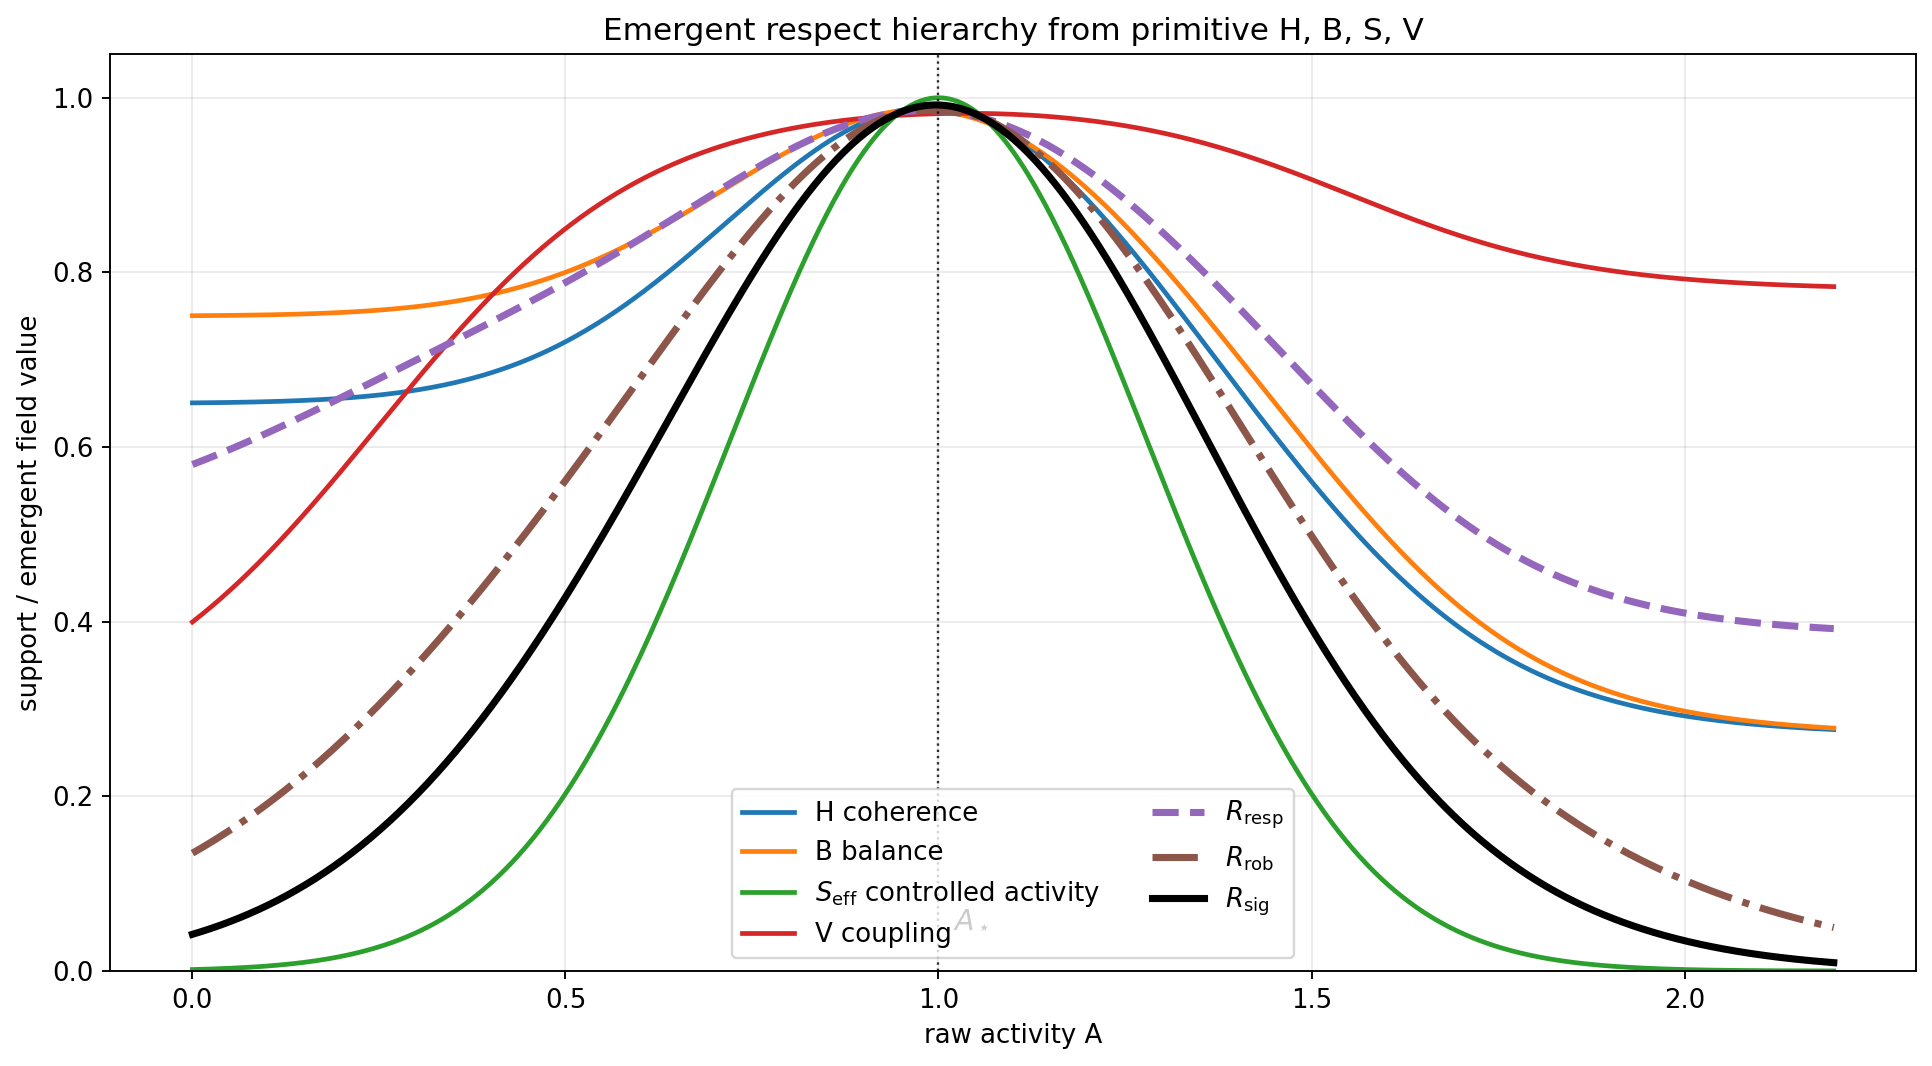
\includegraphics[width=0.98\linewidth]{fig1_respect_hierarchy_vs_activity.png}
\caption{Emergent respect hierarchy as a function of raw activity.
Passive adherence can be nonzero at low activity, but active significance
peaks only near the controlled-activity window.}
\label{fig:hierarchy}
\end{figure}

\begin{figure}[H]
\centering
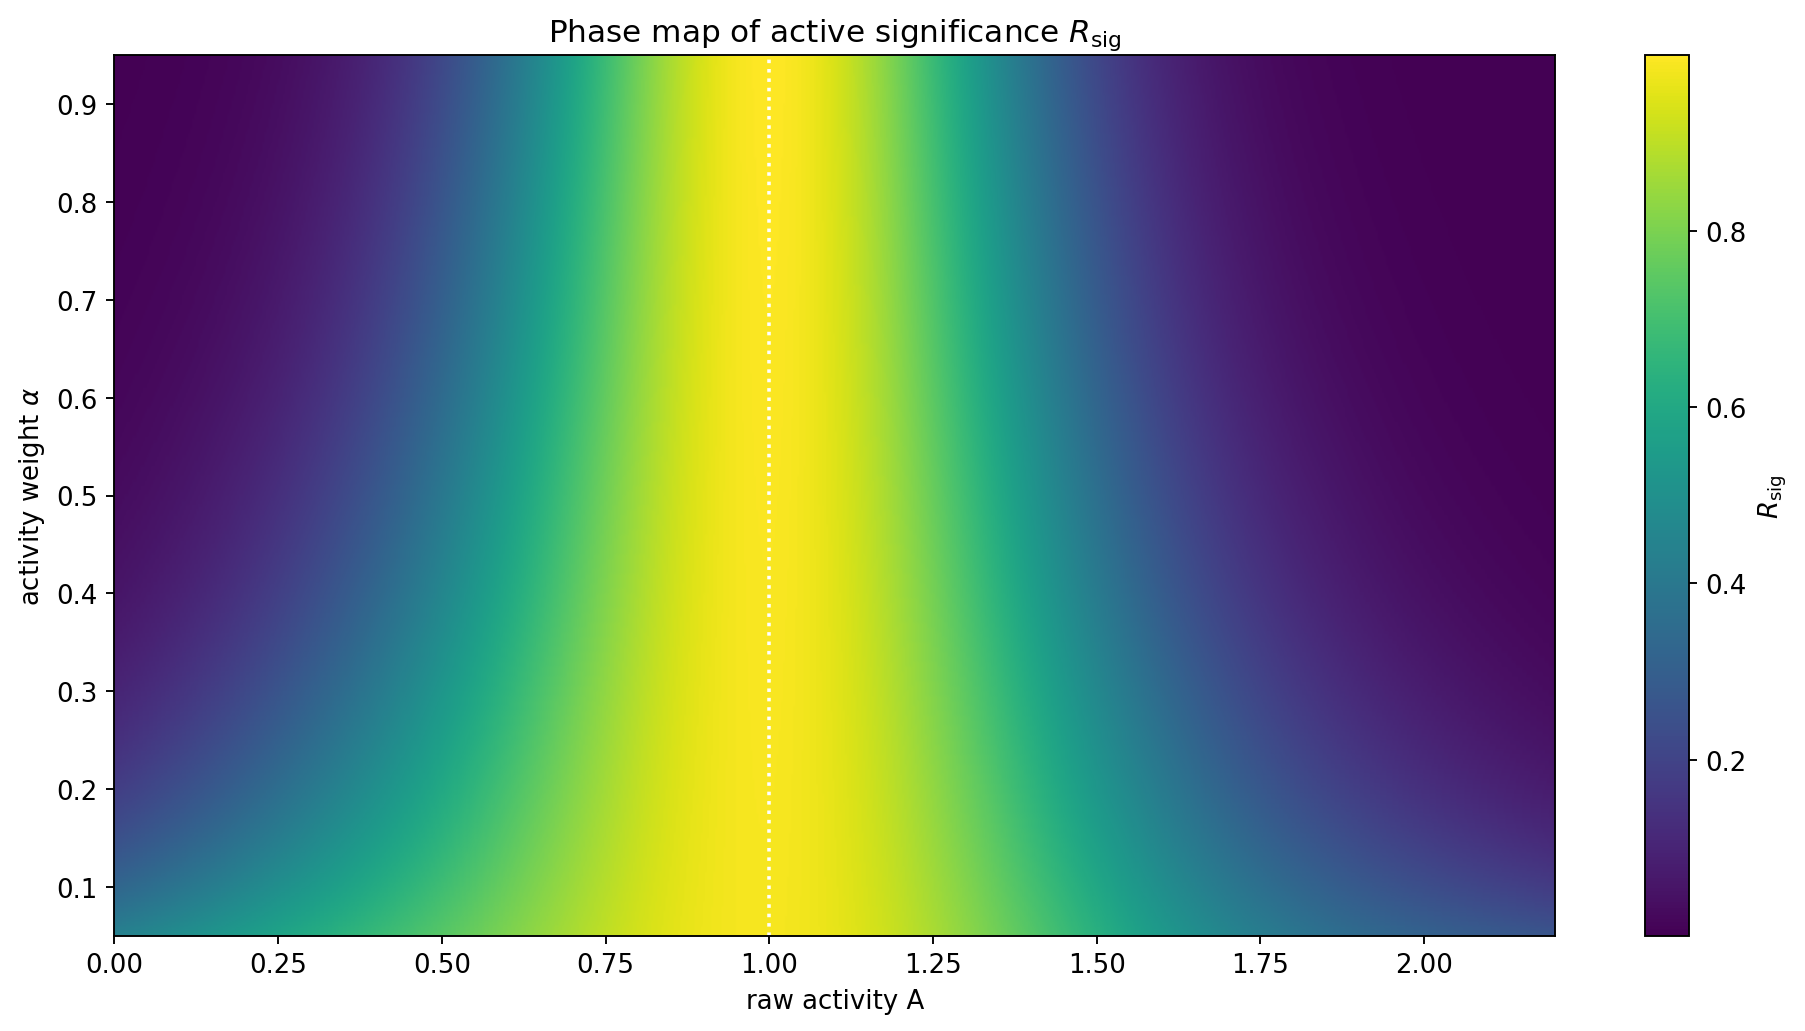
\includegraphics[width=0.95\linewidth]{fig2_rsig_phase_map.png}
\caption{Phase map of $\Rsig$ over raw activity $A$ and activity weight
$\alpha$.
The high-significance ridge is localised near $A_\star=1$.}
\label{fig:phase}
\end{figure}

\begin{figure}[H]
\centering
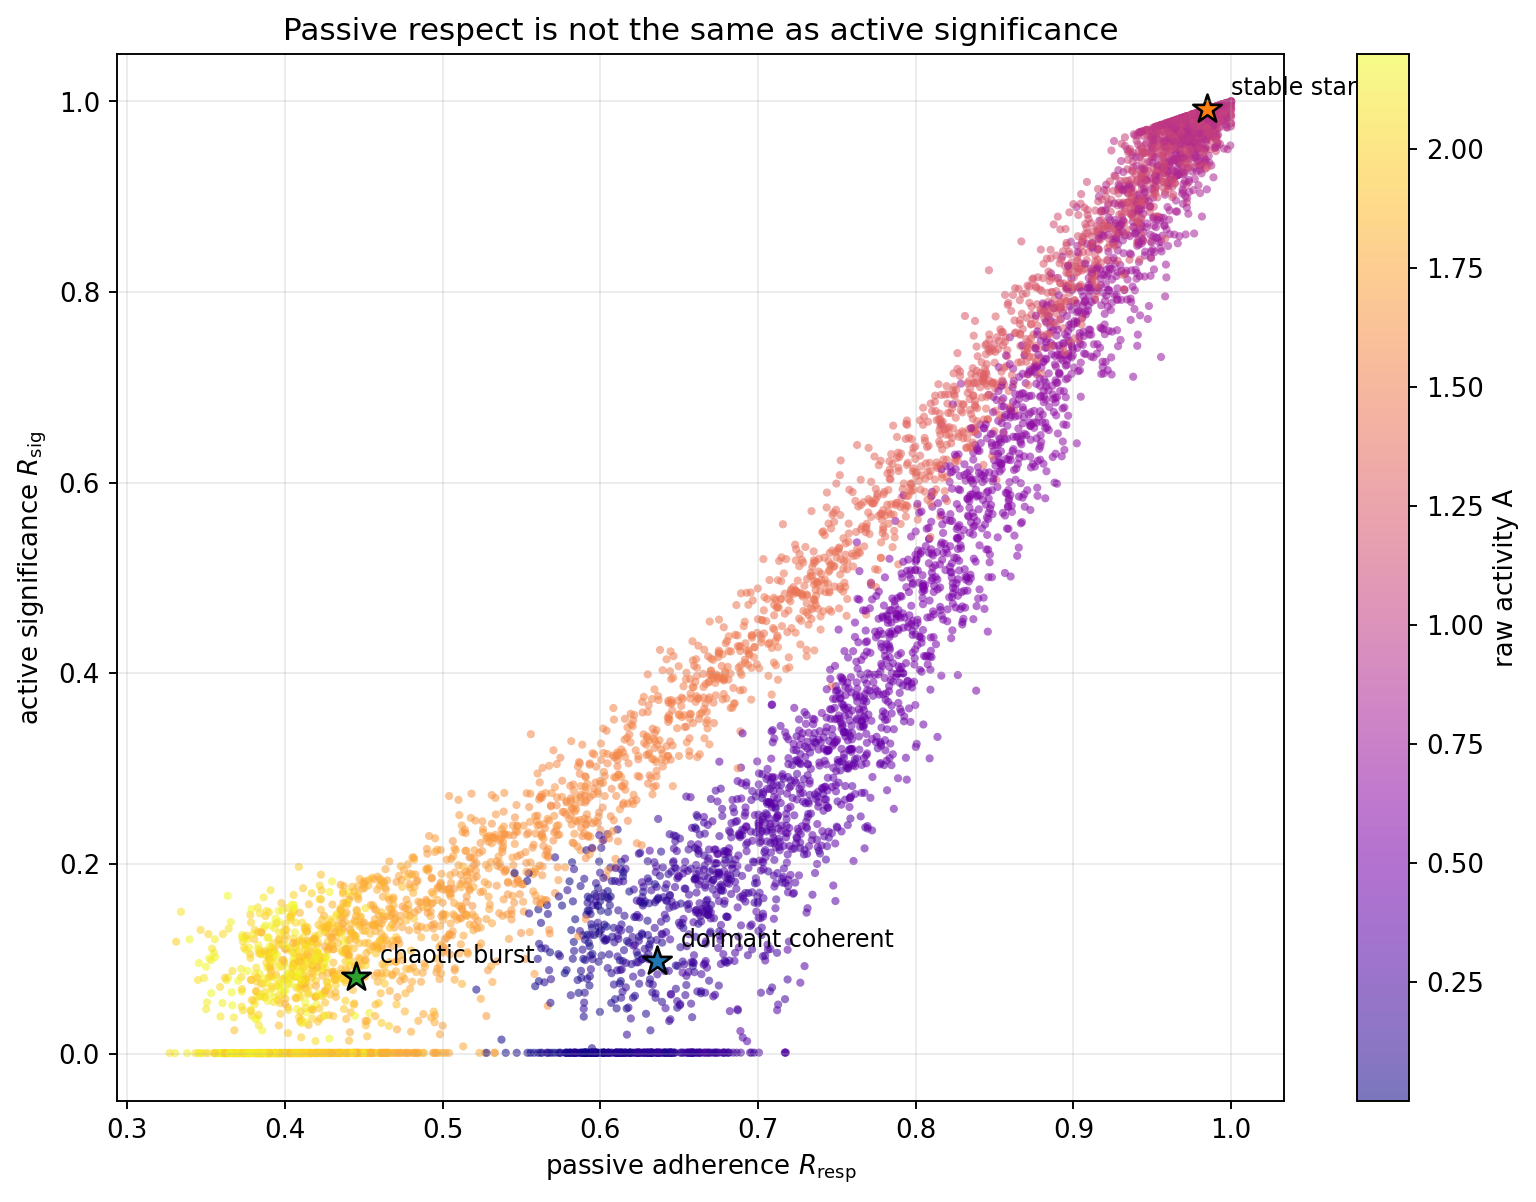
\includegraphics[width=0.86\linewidth]{fig3_passive_vs_active_significance.png}
\caption{Passive respect is not active significance.
Dormant coherent configurations may have moderate $\Rresp$ while remaining
low in $\Rsig$.
The stable-star archetype occupies the high-adherence/high-significance
region.}
\label{fig:scatter}
\end{figure}

\begin{figure}[H]
\centering
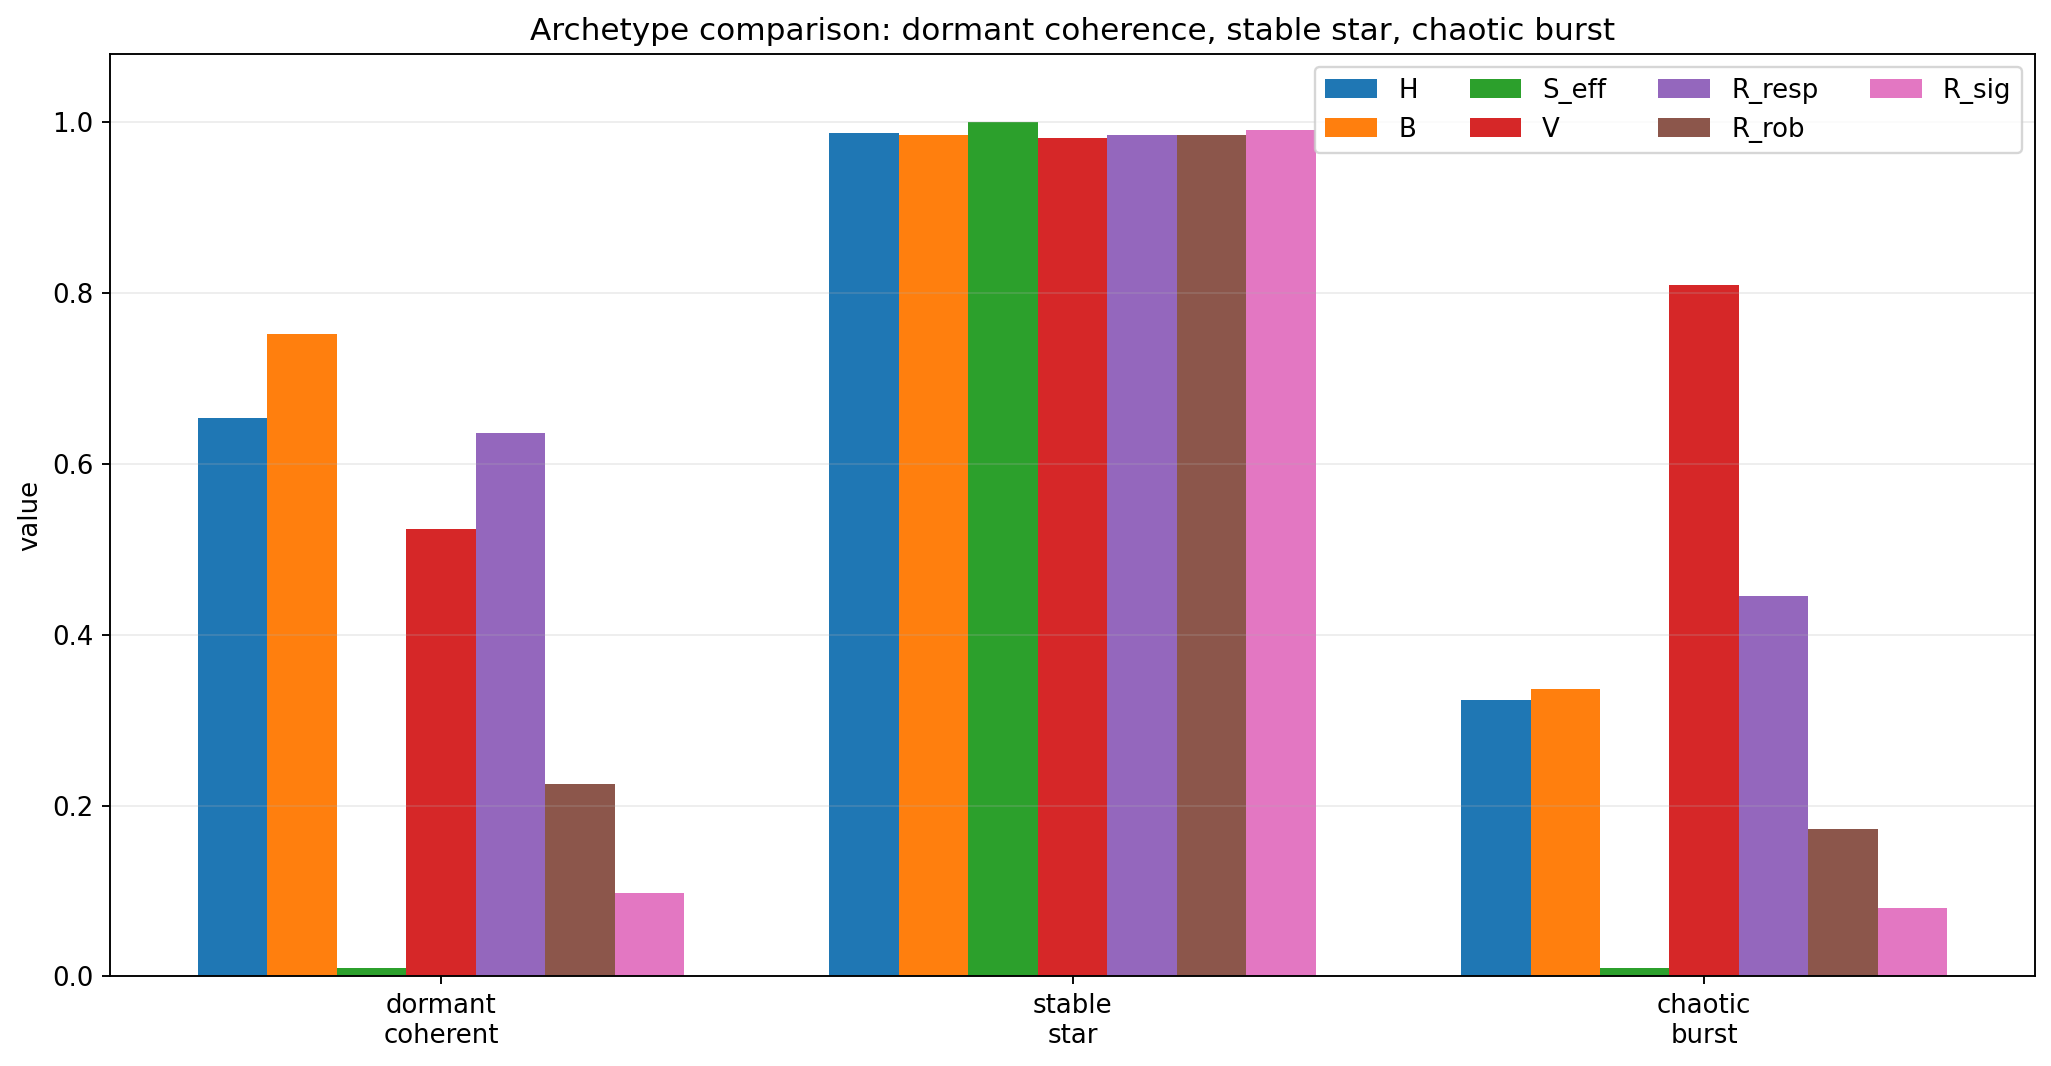
\includegraphics[width=0.95\linewidth]{fig4_archetype_supports.png}
\caption{Archetype comparison.
The stable-star state combines high coherence, balance, controlled activity,
connectedness, robustness, and active significance.}
\label{fig:archetypes}
\end{figure}

% ------------------------------------------------------------
\section{Interpretation}

The simulation supports the following interpretation:
\[
\boxed{
R\;\text{is not absent and not primitive; it is emergent and layered.}
}
\]
In particular,
\begin{align}
\Rresp &:\quad \text{passive structural adherence},\\
\Rrob  &:\quad \text{activity-sensitive robustness},\\
\Rsig  &:\quad \text{active structural significance}.
\end{align}

This preserves the v1.2.1 architecture.
The four primary sectors remain
\[
H,\;B,\;S,\;V.
\]
The new object $\Rsig$ is a candidate diagnostic extension, not an additional
primary field and not an additional freely fitted sector weight.

The star-like interpretation is useful.
A star is not significant merely because it is stable.
It becomes structurally significant because coherent order, hydrostatic
balance, controlled energy production, and environmental coupling jointly
produce persistent influence.
The stable-star label is used as an archetypal metaphor for controlled
energy-producing structure, not as an astrophysical stellar model.

% ------------------------------------------------------------
\section{Limitations}

\begin{itemize}[leftmargin=1.5em]
\item The simulation is a toy model, not a physical stellar model.
\item The support functions $H(A)$, $B(A)$, and $V(A)$ are phenomenological.
\item The parameters $A_\star$, $\sigma_A$, and $\alpha$ are illustrative.
\item No empirical calibration of $\Rsig$ is performed.
\item The result does not modify the v1.2.1 robustness closure used in
Papers 36--43.
\end{itemize}

% ------------------------------------------------------------
\section{Reproducibility}

The numerical pipeline is contained in the public repository:
\begin{center}
\url{https://github.com/Chris4081/structural-selection-principle}
\end{center}

The experiment folder is:
\begin{center}
\texttt{experiments/active\_respect\_significance/}
\end{center}

Run:
\begin{verbatim}
python3 active_respect_significance.py
\end{verbatim}

The script generates:
\begin{itemize}[leftmargin=1.5em]
\item \texttt{outputs/active\_respect\_significance\_results.json},
\item \texttt{outputs/active\_respect\_curves.csv},
\item \texttt{outputs/active\_respect\_ensemble.csv},
\item \texttt{outputs/fig1\_respect\_hierarchy\_vs\_activity.png},
\item \texttt{outputs/fig2\_rsig\_phase\_map.png},
\item \texttt{outputs/fig3\_passive\_vs\_active\_significance.png},
\item \texttt{outputs/fig4\_archetype\_supports.png}.
\end{itemize}

The random seed is fixed to $42$.

% ------------------------------------------------------------
\section{Conclusion}

Paper 44 introduces a minimal toy extension of the MAAT v1.2.1 robustness
closure.
It does not return to a fifth primitive $R$ sector.
Instead, it separates passive adherence, activity-sensitive robustness, and
active structural significance.

The toy simulation shows that passive adherence can remain nonzero in dormant
coherent systems, while active significance peaks only when activity is
controlled and structurally integrated.
This resolves a conceptual tension in the interpretation of $R$:
respect/robustness is real, but it is best treated as an emergent hierarchy
over $H,B,S,V$ rather than as a primitive field.

\begin{thebibliography}{99}

\bibitem{paper36}
C.~Krieg,
``The Maturation of MAAT: From Projection Diagnostics to Emergent Robustness
Closure,''
preprint (2026).

\bibitem{paper41}
C.~Krieg,
``MAAT v1.2.1 Variable Closure and Measurement Definitions,''
preprint (2026).

\bibitem{paper43}
C.~Krieg,
``Linear Perturbations and Structure Growth,''
preprint (2026).

\bibitem{Haken1983}
H.~Haken,
\emph{Synergetics: An Introduction},
Springer (1983).

\bibitem{Goldenfeld1992}
N.~Goldenfeld,
\emph{Lectures on Phase Transitions and the Renormalization Group},
Addison-Wesley (1992).

\end{thebibliography}

\end{document}
